\documentclass{article}
\usepackage[T1]{fontenc}
\usepackage{lmodern}
\usepackage{graphicx}
\usepackage{amsmath,amssymb}
\usepackage[a4paper,margin=2cm]{geometry}
\usepackage[absolute,overlay]{textpos}
\setlength{\TPHorizModule}{1mm}
\setlength{\TPVertModule}{1mm}
\usepackage[indonesian]{babel}
\usepackage{hyperref}
\setlength{\emergencystretch}{2em}
% unit: Halaman 103

\begin{document}

% === Halaman 103 (llm) ===

\begin{itemize}
    \item Dekripsi:
\end{itemize}

\[ P = K^{-1} C \]

Cipherteks: $\text{LNS}$ atau $\text{C} = (11, 13, 18)$

\vspace{10mm}

Plainteks: $\begin{pmatrix} 4 & 9 & 15 \\ 15 & 17 & 6 \\ 24 & 0 & 17 \end{pmatrix} \begin{pmatrix} 11 \\ 13 \\ 18 \end{pmatrix} = \begin{pmatrix} 431 \\ 494 \\ 570 \end{pmatrix} \pmod{26} = \begin{pmatrix} 15 \\ 0 \\ 24 \end{pmatrix}$

\vspace{10mm}

$\text{C} = (15, 0, 24) = (\text{P, A, Y})$

% deskripsi: Perhitungan matriks dekripsi Hill Cipher dari cipherteks ke plainteks
% bbox normalisasi: [0.2550, 0.5220, 0.7470, 0.7410]
\begin{textblock*}{103.32mm}(53.55mm,155.03mm)
\noindent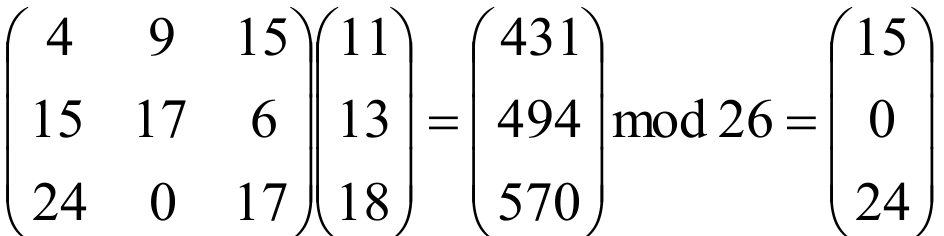
\includegraphics[width=103.32mm,height=65.04mm]{../../images/llm/page_103_img_01.png}%
\end{textblock*}

\end{document}
